\documentclass[aspectratio=1609,ADDITIONAL_DOCCLASS_ARGS]{beamer}

\usetheme[title style=centered, footerstyle=progress, tikzlines]{kth}
\usefonttheme{kth}

\usepackage{bm}
\usepackage{xcolor}
\usepackage[outputdir=_build]{minted}

\colorlet{mathcolor1}{blue!60!green}
\newcommand{\tcolorbf}[2]{\textbf{\textcolor{#1}{#2}}}
\newcommand{\mcolorbf}[2]{\bm{\textcolor{#1}{#2}}}
\newcommand{\tcolor}[2]{\textcolor{#1}{#2}}
\newcommand{\mcolor}[2]{\textcolor{#1}{#2}}

\title{Deep RL with PyTorch and Gymnasium}

\author{\parbox[t][5mm][c]{5cm}{\centering John Wikman\\\small{\texttt{jwikman@kth.se}}\vspace{5mm}}}
\institute{KTH Royal Institute of Technology}
\date{2023-10-31}

\AtBeginSubsection[]
{
  \begin{frame}<beamer>{Outline}
    \tableofcontents[currentsection,currentsubsection]
  \end{frame}
}
\begin{document}


\frame[plain, t]{\titlepage}


\begin{frame}{What to Expect}
  \begin{itemize}
  \setlength\itemsep{2mm}
  \item<1-> Only formulas and notation only necessary for the
        implementation. Warm-up before going through the code.
  \item<2-> \textbf{Will gloss over A LOT of theory.}
  \item<3-> See the book by Sutton and Barto (theory) and DQN Paper:
  {\small
        \begin{thebibliography}{10}

        \beamertemplatebookbibitems

        \bibitem{book:2018:rl}
          Richard S. Sutton and Andrew G. Barto
          \newblock {\em Reinforcement Learning, An Introduction}.
          \newblock The MIT Press, 2018.
          \vspace{1mm}
          \newblock Available for free online:
          \newblock \url{http://incompleteideas.net/book/RLbook2020.pdf}

        \beamertemplatearticlebibitems

        \bibitem{art:2013:dqn}
          Mnih V., Kavukcuoglu K., Silver D., Graves A., Antonoglou I., Wierstra D., Riedmiller M.
          \newblock {\em Playing Atari with Deep Reinforcement Learning}.
          \newblock NIPS Deep Learning Workshop 2013
          \newblock \url{http://arxiv.org/abs/1312.5602}
        \end{thebibliography}
  }
  \end{itemize}
\end{frame}

\begin{frame}{Outline}
  \tableofcontents
\end{frame}

\section{Recap of Reinforcement Learning}
\subsection{What are we optimizing?}

\begin{frame}{The Agent and the Environment}
  \begin{columns}
    \column{0.64\textwidth}
      \begin{itemize}
      \setlength\itemsep{2mm}
      \item<1-> Know state space $s \in S$ and action space $a \in A$.
      \item<2-> Functions $p(s'|s,a)$ and $r(s,a)$ assumed unknown, only observe
            their output in transitions $(s, a, r, s')$.
      \item<3-> Policy performance metric, the Q-function.
      \item<4-> $Q^\pi(s,a)$: \emph{How good is action $a$ in state $s$ on policy $\pi$?}
            \[
            Q^\pi(s,a) = \begin{cases}
            r(s,a) + \gamma \mathbb{E}_{s' \sim p(\cdot|s,a), a' \sim \pi(\cdot|s')} \left[
                Q^\pi(s',a')
            \right]
            \\
            r(s,a) \text{\hspace{5mm} if } s' \text{ is terminal}
            \end{cases}
            \]
            \begin{itemize}
            \item The \emph{discount} $0 < \gamma < 1$ ensures convergence
            \end{itemize}

      \item<5-> $Q^*(s,a)$: \emph{How good is $a$ in $s$ under an optimal policy?}
      \end{itemize}
    \column{0.35\textwidth}
      \begin{figure}
        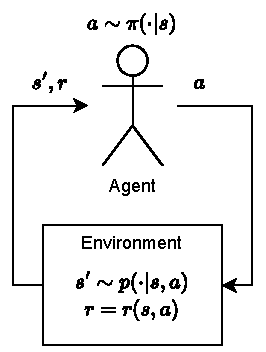
\includegraphics[width=0.65\textwidth]{img/agent-env.pdf}
        \caption{Agent-Env Interaction}
      \end{figure}
  \end{columns}
\end{frame}

\begin{frame}{Q-Function Approximator}
  \begin{itemize}
  \setlength\itemsep{2mm}
  \item<1-> If known $Q^*(s,a)$, then $\arg\max_a Q^*(s,a)$ will most likely give an optimal policy
  \item<2-> Cannot compute $Q^*(s,a)$ since we do not know $p(s'|s,a)$ and
        $r(s,a)$
  \item<3-> But can estimate it over observations $(s,a,r,s')$:
        \hspace{1mm} {\scriptsize\em (equal on average)}
        \begin{equation}
        Q^*(s,a) \approx r + \gamma Q(s', \arg\max_{a'} Q^*(s', a'))
        \end{equation}
  \item<4-> \underline{If finite $A$}, parameterized function
        $f_\theta(s) : \mathbb{R}^d \times S \rightarrow \mathbb{R}^{|A|}$
        can estimate $Q^*(s,a)$ as
        \begin{equation}
        f_\theta(s) \approx [Q^*(s,a_0), Q^*(s,a_1), ..., Q^*(s,a_{|A|-1})]
        \end{equation}
  \item<5-> \textbf{Benefit:} $f_\theta(s)$ allows for trivial argmax
  \item<6-> Will use notation $Q_\theta(s,a) = f_\theta(s)[a]$ from now on
  \end{itemize}
\end{frame}

\begin{frame}{Learning the Q-Function}
  \begin{itemize}
  \setlength\itemsep{2mm}
  \item<1-> Recall what we want to approximate:
        \begin{equation}
        Q_\theta(s,a) \approx Q^*(s,a) = r + \gamma Q(s', \arg\max_{a'} Q^*(s', a'))
        \end{equation}
  \item<2-> Substitute and subtract to get the approximation error:
        \begin{equation}
        err =
        \mcolor{mathcolor1}{r + \gamma Q_\theta(s', \arg\max_{a'} Q_\theta(s', a'))}
        - Q_\theta(s,a)
        \end{equation}
  \item<3-> We denote $\mcolor{mathcolor1}{r + \gamma Q_\theta(s', \arg\max_{a'} Q_\theta(s', a'))}$ as the \tcolorbf{mathcolor1}{target} that $Q_\theta(s,a)$ should approximate.
  \end{itemize}
\end{frame}

\begin{frame}{Exploring the Environment}
  \begin{itemize}
  \setlength\itemsep{2mm}
  \item<1-> \textbf{Catch 22:}
        \begin{enumerate}
        \setlength\itemsep{2mm}
        \item<2-> Get a policy by probing $Q^*(s,a)$
        \item<3-> Approximate $Q^*(s,a)$ by observing transitions
        \item<4-> Observe transition by acting on the policy
        \end{enumerate}
  \item<5-> \textbf{Solution: Bootstrapping with $\epsilon$-greedy policy}
        \begin{itemize}
        \setlength\itemsep{2mm}
        \item<6-> Start with some function $Q_\theta(s,a)$
        \item<7-> With a small probability $\epsilon$, choose a random action
        \item<8-> Otherwise act by $\arg\max_a Q_\theta(s,a)$
        \end{itemize}
  \item<9-> As we observe more data, $Q_\theta(s,a)$ should become more accurate,
        which gives better actions, which hopefully converges to an optimal
        policy.\\[1mm]\emph{\small(No guarantees in this setting.)}
  \end{itemize}
\end{frame}

\subsection{Deep Q-Learning}

\begin{frame}{Deep Q-Learning (DQN)}
  \begin{itemize}
  \setlength\itemsep{2mm}
  \item<1-> $Q_\theta(s, a)$ is represented as a neural network.
  \item<2-> Split into two networks, the training network $\theta$ and the
        \tcolorbf{mathcolor1}{target} network $\bar{\theta}$.
  \item<3-> Optimize by gradient descent of the Mean Squared Error (MSE) of
        training estimate and the target estimate
        \begin{equation}
        \theta \leftarrow \theta -
        \alpha \nabla_\theta \mathbb{E}_{(s,a,r,s') \sim B}\left[\left(
          \mcolor{mathcolor1}{r + \gamma Q_{\bar{\theta}}(s', \arg\max_{a'} Q_{\bar{\theta}}(s', a'))}
          - Q_\theta(s,a)
        \right)^2\right]
        \end{equation}
        where $\alpha$ is the learning rate and $B$ is a replay memory of
        previous interactions.
  \item<4-> Every so often, update target weights: $\bar{\theta} \leftarrow \theta$
  \end{itemize}
\end{frame}

\section{Practical RL Tools}
\subsection{Overview}

\begin{frame}{Overview of RL Tools in Practice}
  \begin{itemize}
  \setlength\itemsep{2mm}
  \item<1-> Python is standard in ML, but often just a wrapper around optimized
        low-level code
  \item<2-> Tools that cover three aspects of RL: \emph{environments},
        \emph{learning}, and \emph{statistics}. Examples:
        \begin{itemize}
        \item Environments: \textbf{Gymnasium}
        \item Learning: \textbf{PyTorch}
        \item Statistics: \textbf{TensorBoard}
        \end{itemize}
  \item<3-> Will briefly cover Gymnasium on the next slide. PyTorch and TensorBoard
        only shown in practice.
  \end{itemize}
\end{frame}


\AtBeginSubsection[]{}

\subsection{Gymnasium}

\begin{frame}{Gymnasium}{Overview}
  \begin{itemize}
  \setlength\itemsep{2mm}
  \item<1-> A standardized API for RL interaction
  \item<2-> Provides a set of standard environments
        \begin{itemize}
        \item Analogous to MNIST, CIFAR-10 (etc.) datasets for supervised learning
        \end{itemize}
  \item<3-> Originally provided by OpenAI
  \item<4-> Recently handed off to the Farama Foundation\\
        \url{https://gymnasium.farama.org}
  \end{itemize}
\end{frame}

\begin{frame}[fragile]{Gymnasium}{Interface example}
\begin{minted}{python}
import gymnasium as gym
env = gym.make("Pendulum-v1") # Off-the-shelf environment

s, _ = env.reset() # Reset environment, get initial state
while True:
  a = your_policy(s) # pi(a|s)

  # Observe p(s'|s,a) and r(s,a) from environment
  s_next, r, terminated, truncated, _ = env.step(a)
  if terminated or truncated:
    break

  s = s_next
\end{minted}
\end{frame}

\end{document}


